\chapter{OTA - Exercício 3 - Analíticos} \label{Chap:AppendixAnaliticosA03}

%CASO 1
\begin{xltabular}{\textwidth}{|l|X|X|}
	\hline
	\endfirsthead
	
	\hline \multicolumn{3}{|c|}{continuação da página anterior} \\ \hline
	\endhead
	
	\hline \multicolumn{3}{|r|}{Continua na próxima página} \\ \hline
	\endfoot
	
	\hline
	\endlastfoot
	
	\multicolumn{3}{|c|}{\cellcolor[HTML]{C0C0C0}\textbf{CASO DE TESTE 1}} \\ \hline


%	\multicolumn{3}{|c|}{\cellcolor[HTML]{DEDEDE}\textbf{Nota Ponderada - EF1}} \\ \hline
	\multicolumn{3}{|c|}{\textbf{Blocos}} \\ \hline
	\multicolumn{3}{|l|}{\begin{tabular}[c]{@{}l@{}} \\ 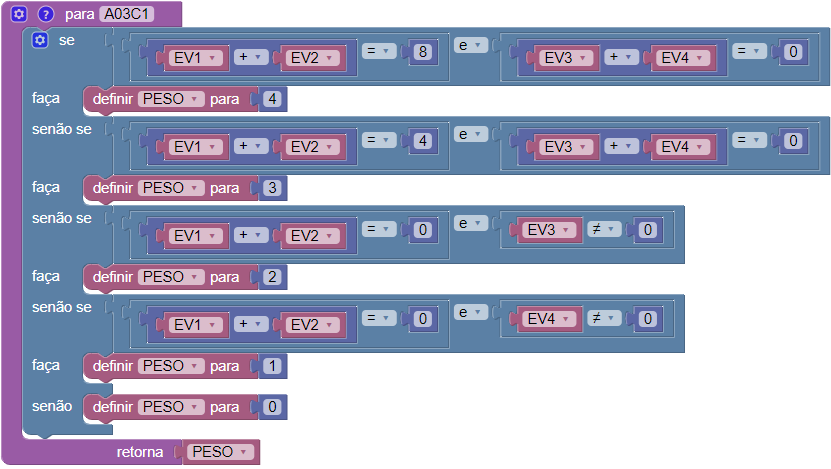
\includegraphics[width=0.9\linewidth]{chapters/appendixAnalytics/A03/C1.png}  \end{tabular}
	} \\ \hline
	\multicolumn{3}{|c|}{\textbf{Python gerado}} \\ \hline
	\multicolumn{3}{|l|}{ \begin{tabular}[c]{@{}l@{}}import math \\ def A03C1():\\ \quad global PESO, EV3, EV4, EV1, EV2\\ \quad if EV1 + EV2 == 8 and EV3 + EV4 == 0:\\ \qquad PESO = 4\\ \quad elif EV1 + EV2 == 4 and EV3 + EV4 == 0:\\ \qquad PESO = 3\\ \quad elif EV1 + EV2 == 0 and EV3 != 0:\\ \qquad PESO = 2\\ \quad elif EV1 + EV2 == 0 and EV4 != 0:\\ \qquad PESO = 1\\ \quad else:\\ \qquad PESO = 0\\ \quad return PESO\end{tabular} }\\ \hline
	
\end{xltabular}

\pagebreak

%CASO 2
\begin{xltabular}{\textwidth}{|l|X|X|}
	\hline
	\endfirsthead
	
	\hline \multicolumn{3}{|c|}{continuação da página anterior} \\ \hline
	\endhead
	
	\hline \multicolumn{3}{|r|}{Continua na próxima página} \\ \hline
	\endfoot
	
	\hline
	\endlastfoot
	
	\multicolumn{3}{|c|}{\cellcolor[HTML]{C0C0C0}\textbf{CASO DE TESTE 2}} \\ \hline
	
%	\multicolumn{3}{|c|}{\cellcolor[HTML]{DEDEDE}\textbf{Nota Ponderada - EF1}} \\ \hline
	\multicolumn{3}{|c|}{\textbf{Blocos}} \\ \hline
	\multicolumn{3}{|l|}{\begin{tabular}[c]{@{}l@{}} \\ 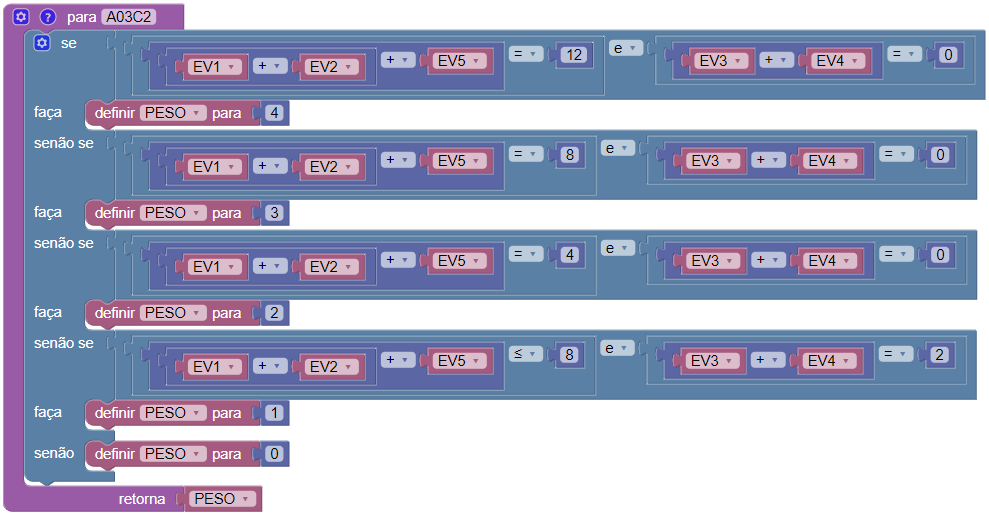
\includegraphics[width=0.9\linewidth]{chapters/appendixAnalytics/A03/C2.png}  \end{tabular}
	} \\ \hline
	\multicolumn{3}{|c|}{\textbf{Python gerado}} \\ \hline
	\multicolumn{3}{|l|}{ \begin{tabular}[c]{@{}l@{}}import math \\ def A03C2():\\ \quad global PESO, EV5, EV3, EV4, EV1, EV2\\ \quad if (EV1 + EV2) + EV5 == 12 and EV3 + EV4 == 0:\\ \qquad PESO = 4 \\ \quad elif (EV1 + EV2) + EV5 == 8 and EV3 + EV4 == 0:\\ \qquad PESO = 3\\ \quad elif (EV1 + EV2) + EV5 == 4 and EV3 + EV4 == 0:\\ \qquad PESO = 2\\ \quad elif (EV1 + EV2) + EV5 <= 8 and EV3 + EV4 == 2:\\ \qquad PESO = 1\\ \quad else:\\ \qquad PESO = 0\\ \quad return PESO \end{tabular} }\\ \hline
	
\end{xltabular}

\pagebreak
%CASO 3
\begin{xltabular}{\textwidth}{|l|X|X|}
	\hline
	\endfirsthead
	
	\hline \multicolumn{3}{|c|}{continuação da página anterior} \\ \hline
	\endhead
	
	\hline \multicolumn{3}{|r|}{Continua na próxima página} \\ \hline
	\endfoot
	
	\hline
	\endlastfoot
	
	\multicolumn{3}{|c|}{\cellcolor[HTML]{C0C0C0}\textbf{CASO DE TESTE 3}} \\ \hline
	
	%EF1
%	\multicolumn{3}{|c|}{\cellcolor[HTML]{DEDEDE}\textbf{Nota Ponderada - EF1}} \\ \hline
	\multicolumn{3}{|c|}{\textbf{Blocos}} \\ \hline
	\multicolumn{3}{|l|}{\begin{tabular}[c]{@{}l@{}} \\ 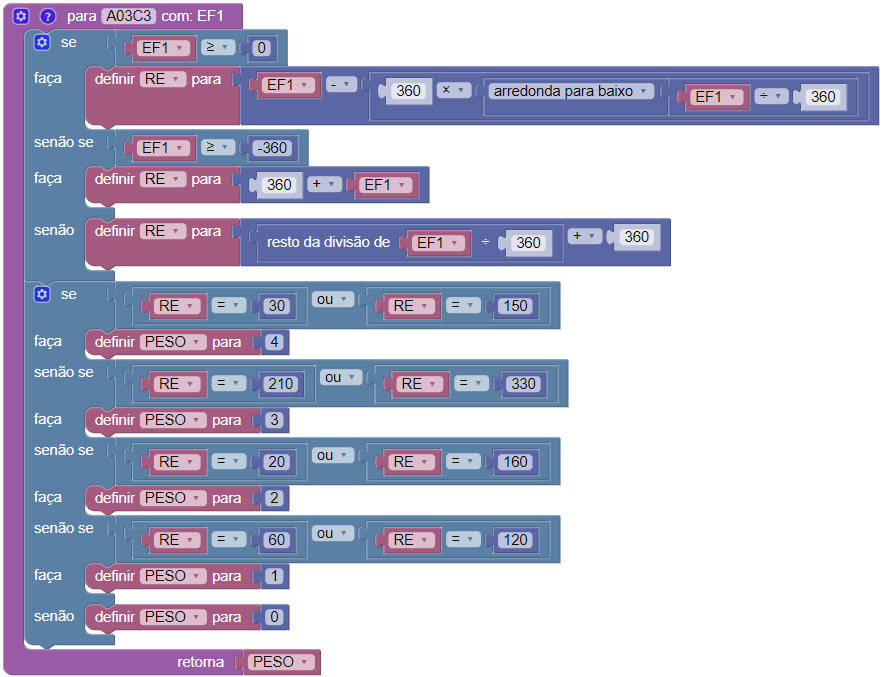
\includegraphics[width=0.9\linewidth]{chapters/appendixAnalytics/A03/C3.png}  \end{tabular}
	} \\ \hline
	\multicolumn{3}{|c|}{\textbf{Python gerado}} \\ \hline
	\multicolumn{3}{|l|}{ \begin{tabular}[c]{@{}l@{}}import math \\ \# Nota Ponderada - EF1 - Caso 3\\ def A03C3(EF1):\\ \quad global PESO, RE\\ \quad if EF1 >= 0:\\ \qquad RE = EF1 - 360 * math.floor(EF1 / 360)\\ \quad elif EF1 >= -360:\\ \qquad RE = 360 + EF1\\ \quad else:\\ \qquad RE = EF1 \% 360 + 360\\ \quad if RE == 30 or RE == 150:\\ \qquad PESO = 4\\ \quad elif RE == 210 or RE == 330:\\ \qquad PESO = 3\\ \quad elif RE == 20 or RE == 160:\\ \qquad PESO = 2\\ \quad elif RE == 60 or RE == 120:\\ \qquad PESO = 1\\ \quad else:\\ \qquad PESO = 0\\ \quad return PESO \end{tabular} }\\ \hline
	
\end{xltabular}

\pagebreak
%CASO 4
\begin{xltabular}{\textwidth}{|l|X|X|}
	\hline
	\endfirsthead
	
	\hline \multicolumn{3}{|c|}{continuação da página anterior} \\ \hline
	\endhead
	
	\hline \multicolumn{3}{|r|}{Continua na próxima página} \\ \hline
	\endfoot
	
	\hline
	\endlastfoot
	
	\multicolumn{3}{|c|}{\cellcolor[HTML]{C0C0C0}\textbf{CASO DE TESTE 4}} \\ \hline
	
	%EF1
%	\multicolumn{3}{|c|}{\cellcolor[HTML]{DEDEDE}\textbf{Nota Ponderada - EF1}} \\ \hline
	\multicolumn{3}{|c|}{\textbf{Blocos}} \\ \hline
	\multicolumn{3}{|l|}{\begin{tabular}[c]{@{}l@{}} \\ 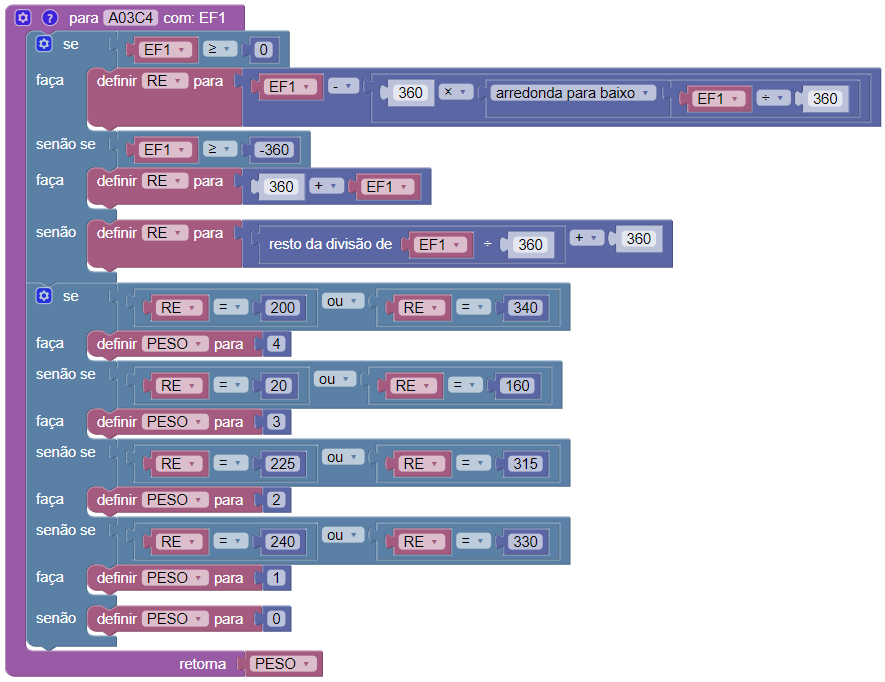
\includegraphics[width=0.9\linewidth]{chapters/appendixAnalytics/A03/C4.png}  \end{tabular}
	} \\ \hline
	\multicolumn{3}{|c|}{\textbf{Python gerado}} \\ \hline
	\multicolumn{3}{|l|}{ \begin{tabular}[c]{@{}l@{}}import math \\ \# Nota Ponderada - EF1 - Caso 4\\ \# Redução ao primeiro quadrante \\ def A03C4(EF1):\\ \quad global PESO, RE\\ \quad if EF1 >= 0:\\ \qquad RE = EF1 - 360 * math.floor(EF1 / 360)\\ \quad elif EF1 >= -360:\\ \qquad RE = 360 + EF1\\ \quad else:\\ \qquad RE = EF1 \% 360 + 360\\ \quad if RE == 200 or RE == 340:\\ \qquad PESO = 4\\ \quad elif RE == 20 or RE == 160:\\ \qquad PESO = 3\\ \quad elif RE == 225 or RE == 315:\\ \qquad PESO = 2\\ \quad elif RE == 240 or RE == 330:\\ \qquad PESO = 1\\ \quad else:\\ \qquad PESO = 0\\ \quad return PESO \end{tabular} }\\ \hline

		
\end{xltabular}

\pagebreak
%CASO 5
\begin{xltabular}{\textwidth}{|l|X|X|}
	\hline
	\endfirsthead
	
	\hline \multicolumn{3}{|c|}{continuação da página anterior} \\ \hline
	\endhead
	
	\hline \multicolumn{3}{|r|}{Continua na próxima página} \\ \hline
	\endfoot
	
	\hline
	\endlastfoot
	
	\multicolumn{3}{|c|}{\cellcolor[HTML]{C0C0C0}\textbf{CASO DE TESTE 5}} \\ \hline
	
	%EF1
%	\multicolumn{3}{|c|}{\cellcolor[HTML]{DEDEDE}\textbf{Nota Ponderada - EF1}} \\ \hline
	\multicolumn{3}{|c|}{\textbf{Blocos}} \\ \hline
	\multicolumn{3}{|l|}{\begin{tabular}[c]{@{}l@{}} \\ 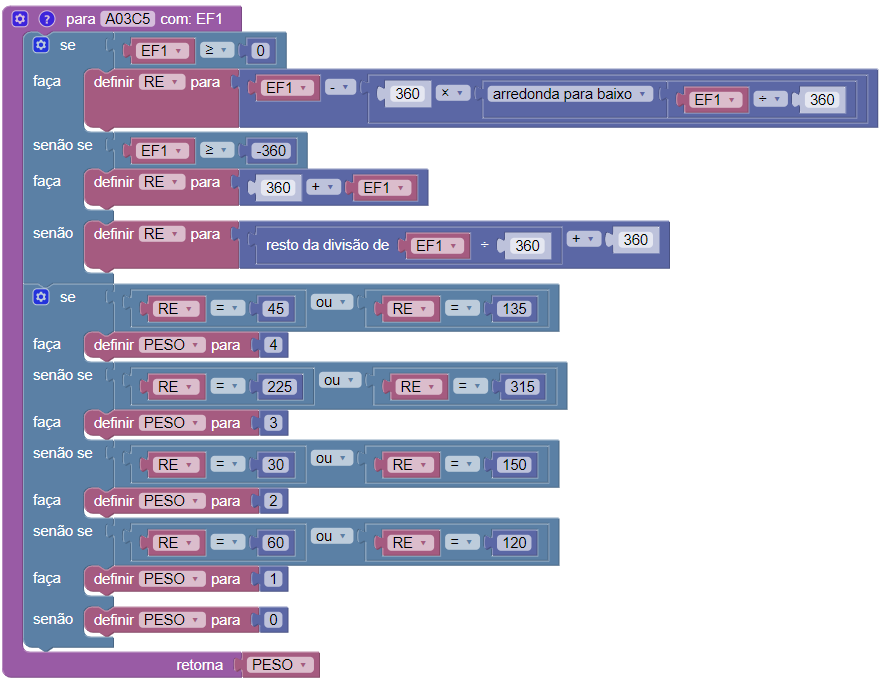
\includegraphics[width=0.9\linewidth]{chapters/appendixAnalytics/A03/C5.png}  \end{tabular}
	} \\ \hline
	\multicolumn{3}{|c|}{\textbf{Python gerado}} \\ \hline
	\multicolumn{3}{|l|}{ \begin{tabular}[c]{@{}l@{}}import math \\ \# Nota Ponderada - EF1 - Caso 5\\ \# Redução ao primeiro quadrante\\ def A03C5(EF1):\\ \quad global PESO, RE\\ \quad if EF1 >= 0:\\ \qquad RE = EF1 - 360 * math.floor(EF1 / 360)\\ \quad elif EF1 >= -360:\\ \qquad RE = 360 + EF1\\ \quad else:\\ \qquad RE = EF1 \% 360 + 360\\ \quad if RE == 45 or RE == 135:\\ \qquad PESO = 4\\ \quad elif RE == 225 or RE == 315:\\ \qquad PESO = 3\\ \quad elif RE == 30 or RE == 150:\\ \qquad PESO = 2\\ \quad elif RE == 60 or RE == 120:\\ \qquad PESO = 1\\ \quad else:\\ \qquad PESO = 0\\ \quad return PESO \end{tabular} }\\ \hline
		
\end{xltabular}

\pagebreak
%CASO 6
\begin{xltabular}{\textwidth}{|l|X|X|}
	\hline
	\endfirsthead
	
	\hline \multicolumn{3}{|c|}{continuação da página anterior} \\ \hline
	\endhead
	
	\hline \multicolumn{3}{|r|}{Continua na próxima página} \\ \hline
	\endfoot
	
	\hline
	\endlastfoot
	
	\multicolumn{3}{|c|}{\cellcolor[HTML]{C0C0C0}\textbf{CASO DE TESTE 6}} \\ \hline
	
	%EF1
%	\multicolumn{3}{|c|}{\cellcolor[HTML]{DEDEDE}\textbf{Nota Ponderada - EF1}} \\ \hline
	\multicolumn{3}{|c|}{\textbf{Blocos}} \\ \hline
	\multicolumn{3}{|l|}{\begin{tabular}[c]{@{}l@{}} \\ 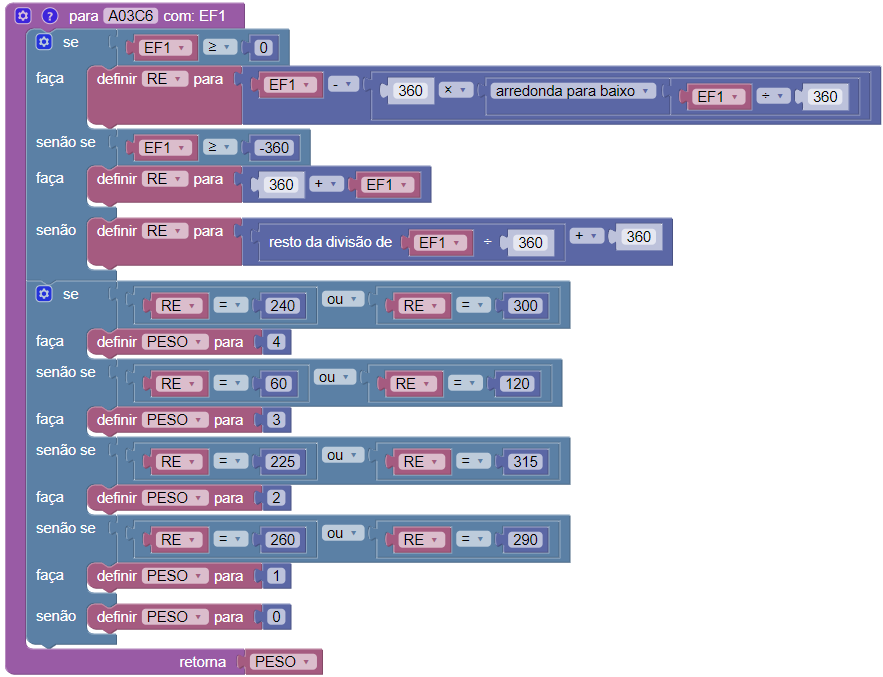
\includegraphics[width=0.9\linewidth]{chapters/appendixAnalytics/A03/C6.png}  \end{tabular}
	} \\ \hline
	\multicolumn{3}{|c|}{\textbf{Python gerado}} \\ \hline
	\multicolumn{3}{|l|}{ \begin{tabular}[c]{@{}l@{}}import math \\ \# Nota Ponderada - EF1 - Caso 6 \\ \# Redução ao primeiro quadrante\\ def EF1CASO6(EF1):\\ \quad global PESO, RE\\ \quad if EF1 >= 0:\\ \qquad RE = EF1 - 360 * math.floor(EF1 / 360)\\ \quad elif EF1 >= -360:\\ \qquad RE = 360 + EF1\\ \quad else:\\ \qquad RE = EF1 \% 360 + 360\\ \quad if RE == 240 or RE == 300:\\ \qquad PESO = 4\\ \quad elif RE == 60 or RE == 120:\\ \qquad PESO = 3\\ \quad elif RE == 225 or RE == 315:\\ \qquad PESO = 2\\ \quad elif RE == 260 or RE == 290:\\ \qquad PESO = 1\\ \quad else:\\ \qquad PESO = 0\\ \quad return PESO \end{tabular} }\\ \hline
	
\end{xltabular}

